\chapter{Estudos de caso}
\label{SectionEstudosDeCaso}
Neste capítulo, será estudado uma rede elementar de 2 barras e 1 linha de transmissão (na seção \ref{SectionRedePequena}) e uma rede maior, de 14 barras e 20 ramos (na seção \ref{SectionRede14barras}). Neste trabalho, a rede elementar tem um papel fundamental para compreensão de cada iteração do método, além de servir como calibração e teste para todas as modificações subsequentes. Para cada modificação no código de referência, ainda que pequena, deve ser retestado tendo a saída desta rede como parâmetro.
\section{Rede de 2 barras e 1 linha de transmissão}
\label{SectionRedePequena}
Considere a rede de duas barras e uma linha de transmissão \ref{FigRede2barras1linha}. Esse é o exemplo mais simples possível e foi apresentado e resolvido nos slides de aula.\\
\begin{figure}[!htb]
\caption{Rede de duas barras e uma linha de transmissão}
 \centering % para centralizarmos a figura
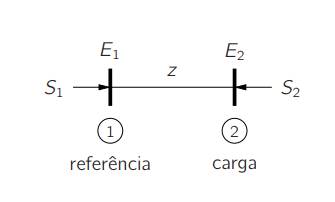
\includegraphics[width=8cm]{figuras/rede2barras1linha.PNG} 
\label{FigRede2barras1linha}
\end{figure}

\begin{equation}
Dados \left\{    \begin{array}{lll}
                E_1=1,0112	\angle 0^o pu\\
                z = 0,01+j0,05 pu\\
                S_2 = -(1,0+j0) pu
            \end{array}\right.
    \label{rede1_dados}
\end{equation}
\subsection{Equacionamento}
A matriz admitância será dada por \ref{rede1_Admitância}, que foi calculado com as regras \ref{AdmitanciaElementosForaDiagonal} e \ref{AdmitanciaElementosDiagonal}.
\begin{equation}
   Y = \left[ 
    \begin{matrix} 
        3,8462-j19,2308 & -3,8462+j19,2308  \\ 
        -3,8462+j19,2308 & 3,8462-j19,2308  
    \end{matrix} \right] 
    \label{rede1_Admitância}
\end{equation}
Portanto, tem-se as equações nodais $P_2$ e $Q_2$ em \ref{PeQ_resolvidos}. As incognitas são $\theta_2$ e $V_2$
\begin{equation}
    \left\{    \begin{array}{lll}
                P_2= V_2V_1(G_{21}cos \theta_{21}+ B_{21}sen \theta_{21}) + V^2_2G_{22}\\
                Q_2= V_2V_1(G_{21}sen \theta_{21}- B_{21}cos \theta_{21}) - V^2_2B_{22}
            \end{array}\right.
    \label{PeQ_resolvidos}
\end{equation}
Portanto, as equações de fluxo serão \ref{PeQ_esp}
\begin{equation}
    \left\{    \begin{array}{lll}
                P^{esp}_2-P_2 = -1-P_2=0\\
                Q^{esp}_2-Q_2 = 0-Q_2=0
            \end{array}\right.
    \label{PeQ_esp}
\end{equation}
Por fim, monta-se as equações linearizadas de fluxo de carga em \ref{FluxoLinearizado}.
\begin{equation}
   \left[ \begin{matrix} \Delta P_2 \\ \Delta Q_2  \end{matrix} \right] =  \left[ \begin{matrix} \frac{\partial (P_2)}{\partial \theta_2} & \frac{\partial (P_2)}{\partial V_2}  \\ \frac{\partial (Q_2)}{\partial \theta_2} & \frac{\partial (Q_2)}{\partial V_2} \end{matrix} \right] .  \left[ \begin{matrix} \Delta \theta_2 \\ \Delta V_2  \end{matrix} \right]
    \label{FluxoLinearizado}
\end{equation}
Onde, a partir de \ref{H_resolvido}, \ref{N_resolvido}, \ref{M_resolvido} e \ref{L_resolvido}, tem-se \ref{HMNL_resolvidoRedePequena}.
\begin{equation}
  \left\{    \begin{array}{llll}
                \frac{\partial (P_2)}{\partial \theta_2} =-V_2 V_1 (G_{21} sen\theta_{21} - B_{21}cos\theta_{21})\\
                \frac{\partial (P_2)}{\partial V_2} =V_1(G_{21} cos\theta_{21} + B_{21}sen\theta_{21}) + 2V_2G_{22}\\
                \frac{\partial (Q_2)}{\partial \theta_2} = V_2 V_1 (G_{21} cos\theta_{21} + B_{21}sen\theta_{21})\\
                \frac{\partial (Q_2)}{\partial V_2} =-V_1 (G_{21} sen\theta_{21} - B_{21}cos\theta_{21})
            \end{array}\right.
    \label{HMNL_resolvidoRedePequena}
\end{equation}
\subsubsection{Processo iterativo $\nu=0$}
Para a primeira iteração ($\nu=0$), tem-se:
\begin{equation}
  \left\{    \begin{array}{llll}
                V_2=1pu\\
                \theta_2=0
    \end{array}\right.
\label{RedePequenaItera0a}
\end{equation}
\begin{equation}
    \left\{    \begin{array}{llll}
                P_2= -0,0431\\
                \Delta P_2 = -0,9569\\
                Q_2 = -0,2154\\
                \Delta Q_2 = 0,2154
            \end{array}\right.
    \label{RedePequenaItera0b}
\end{equation}
Como os mismatches ainda são maiores que a tolerância, atualiza-se o estado, incrementa-se $\nu=\nu+1$. A nova matriz Jacobiana ficará com \ref{JRedePequena}.
\begin{equation}
   J = \left[ 
    \begin{matrix} 
        19,4462 & 3,8031  \\ 
        -3,8031 & 19,0154  
    \end{matrix} \right] 
    \label{JRedePequena}
\end{equation}
\subsubsection{Processo iterativo $\nu=1$}
Para a segunda iteração ($\nu=1$), tem-se:
\begin{equation}
  \left\{    \begin{array}{llll}
                P_2= -0,9960\\
                \Delta P_2 = -0,0040\\
                Q_2 = 0,0240\\
                \Delta Q_2 = -0,0240
            \end{array}\right.
    \label{RedePequenaItera1}
\end{equation}
Como os mismatches ainda são maiores que a tolerância, atualiza-se o estado, incrementa-se $\nu=\nu+1=2$. A nova matriz Jacobiana ficará com \ref{JRedePequena2}.
\begin{equation}
   J = \left[ 
    \begin{matrix} 
        19,2535 & 2,8560  \\ 
        -4,8515 & 19,2781
    \end{matrix} \right] 
    \label{JRedePequena2}
\end{equation}
\subsubsection{Processo iterativo $\nu=2$}
Para a terceira iteração ($\nu=2$), tem-se:
\begin{equation}
  \left\{    \begin{array}{llll}
                P_2= -1\\
                \Delta P_2 = 0\\
                Q_2 = 0\\
                \Delta Q_2 = 0
            \end{array}\right.
    \label{RedePequenaItera2}
\end{equation}
Como os mismatches são menores que a tolerância, o método convergiu.
\subsubsection{Calculo de $E_2$}
Pela equação de potência na barra $2$, tem-se \ref{RedePequenaPotBarra2}.
\begin{equation}
    S_1 = E_1.I^*_12=E1.[\frac{1}{Z}.(E_1-E_2]^*= 1.01+j0,05pu
    \label{RedePequenaPotBarra2}
\end{equation}
Resumo das iterações está aprensentado na tabela \ref{t_redePequenaResumo}.
\begin{table}[!htb]
\centering
\caption{Resumo das iterações da rede}
\begin{tabular}{lll}
\hline
Iteração & $E_2$          & $E_2$ \\ \hline
0        & 1+j0           & $1\angle 0^o$ \\
1        & 1-j0,0494      & $1 \angle -2.84^o$ \\
2        & 0,09988-0,0495 & $1 \angle -2,8^o$ \\ \hline
\end{tabular}
\label{t_redePequenaResumo}
\end{table}

\subsection{Solução por software}
Com os dados \ref{rede1_dados} é possivel montar os \textit{arrays} no código abaixo. Eles serão usados como \textit{inputs} do código utilizado neste trabalho. 
\begin{minted}[mathescape, style = autumn,
    frame = single, fontsize=\footnotesize]{matlab}
nome_da_rede = 'Rede de 2 barras e 1 ramos - Demostração do Slide';
baseMVA      = 1 ; % MVA - Os dados do problema já estavam em pu
%Núm-Tipo-V-Âng-Pg-Qg-Pc-Qc-bshk % (PU/Graus) - 3ref; 2PV; 0PQ
barras = [1 3 1.0112 0 0 0 00.0 0 0
          2 0 0.0000 0 0 0 -1.0 0 0 ];
ramos  = [1 2 0.01 0.05 0.0 1.0 0.0 ];%De-Para-r-x-bshl-tap-fi
\end{minted}
A saída dessa rede, calculado pelo algoritmo descrito no capítulo \ref{SectionCodigo}, é dado nos blocos de código a seguir.
Nesse bloco temos a formação da matriz de admitância. É a mesma matriz calculada em \ref{rede1_Admitância}, como esperado.
\begin{minted}[mathescape, style = autumn,
    frame = single, fontsize=\footnotesize]{matlab}
Y =
3.8462 -19.2308i  -3.8462 +19.2308i
-3.8462 +19.2308i   3.8462 -19.2308i
G =
3.8462   -3.8462
-3.8462    3.8462
B =
-19.2308   19.2308
19.2308  -19.2308
\end{minted}
As iterações e os mismatches estão no próximo bloco
\begin{minted}[mathescape, style = autumn,
    frame = single, fontsize=\footnotesize]{matlab}
> Iteração - 0
  * Máximo mismatch P = 1.0431 (barra 0002)
  * Máximo mismatch Q = 0.2154 (barra 0002)
> Iteração - 1
  * Máximo mismatch P = -0.0268 (barra 0002)
  * Máximo mismatch Q = -0.0291 (barra 0002)
> Iteração - 2
  * Máximo mismatch P = -0.0000 (barra 0002)
  * Máximo mismatch Q = -0.0001 (barra 0002)
\end{minted}
Após 3 iterações, o método convergiu para solução com tolerância de $0,001pu$.
\begin{minted}[mathescape, style = autumn,
    frame = single, fontsize=\footnotesize]{matlab}
> Estado da rede
  Barra Tipo       Mag   Fase         P       Q       Qsh
      1    3    1.0112   0.00   -0.9904  0.0480    0.0000 
      2    0    1.0198   2.78    1.0000  0.0001    0.0000 
> Fluxos de potência
     De Para       Pkm     Qkm       Pmk     Qmk     Ploss   Qloss
      1    2   -0.9904  0.0480    1.0000  0.0001    0.0096  0.0481
> Tempo computacional =  0.0798 segundos.
\end{minted}
Note que na barra $2$, a tensão está como calculado na tabela \ref{t_redePequenaResumo}. $E_2=1 \angle -2,8^o$.



\section{Rede 14 bus IEEE}
\label{SectionRede14barras}
Considere uma rede de 14 barras e 20 ramos. Este exemplo consta no código de referência e também pode ser encontrado no endereço: \href{https://labs.ece.uw.edu/pstca/pf14/pg\_tca14bus.htm}{https://labs.ece.uw.edu/pstca/pf14/pg\_tca14bus.htm}.\\
Neste trabalho não haverá equacionamento manual desta rede pois seria muito extenso. Portanto, apresentaremos dados da simulação.\\
Na figura \ref{FigRede14barras}, há a figura do estudo de caso de rede 14 barras e 20 ramos do IEEE.
\begin{figure}[!htb]
\caption{Rede de 14 barras IEEE}
\centering % para centralizarmos a figura
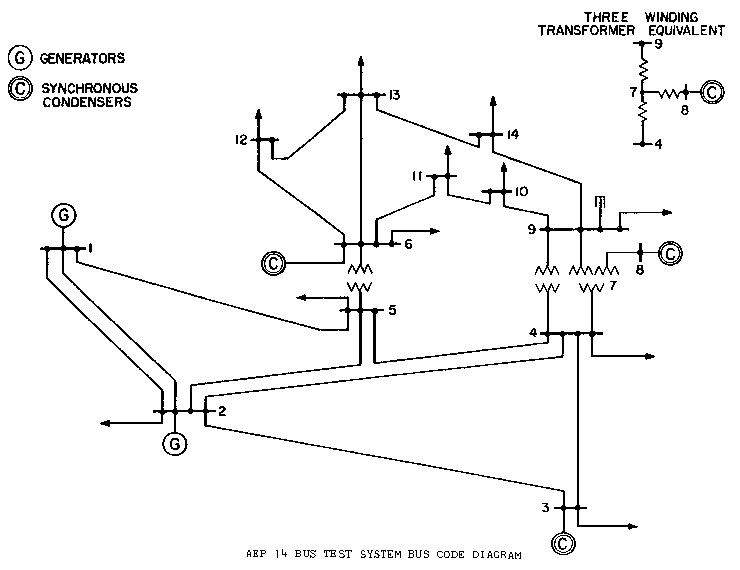
\includegraphics[width=10cm]{figuras/14bus.jpg} 
\label{FigRede14barras}
\end{figure}

\subsection{Entradas do software}
Esta é a tabela de entradas com os parâmetros da rede, que foi disponibilizada pelo IEEE.
\begin{minted}[mathescape, style = autumn,
    frame = single, fontsize=\footnotesize]{matlab}
nome_da_rede = '14 barras IEEE';
baseMVA = 1.0; %pneves já está dividido por 100
%	Número - Tipo - V - Ângulo - Pg - Qg - Pc - Qc - bshk
barras =[ 1   3   1.00   0.00   0.00   0.00  0.00   0.000   0.00
          2   2   1.00   0.00   0.00   0.00  0.217  0.127   0.00
          3   2   1.00   0.00   0.00   0.00  0.942  0.190   0.00
          4   0   1.00   0.00   0.00   0.00  0.478 -0.039   0.00
          5   0   1.00   0.00   0.00   0.00  0.076  0.016   0.00
          6   2   1.00   0.00   0.00   0.00  0.112  0.075   0.00
          7   0   1.00   0.00   0.00   0.00  0.000  0.000   0.00
          8   2   1.00   0.00   0.00   0.00  0.000  0.000   0.00
          9   0   1.00   0.00   0.00   0.00  0.295  0.166   0.19
         10   0   1.00   0.00   0.00   0.00  0.900  0.058   0.00
         11   0   1.00   0.00   0.00   0.00  0.350  0.018   0.00
         12   0   1.00   0.00   0.00   0.00  0.610  0.016   0.00
         13   0   1.00   0.00   0.00   0.00  0.135  0.058   0.00
         14   0   1.00   0.00   0.00   0.00  0.149  0.050   0.00];
%	De - Para - r - x - bshl - tap - fi
ramos=[1    5  0.05403   0.22304     0.0492  1.000  0.00
       1    2  0.01938   0.05917     0.0528  1.000  0.00 
       2    5  0.05695   0.17388     0.0346  1.000  0.00
       2    4  0.05811   0.17632     0.0340  1.000  0.00
       2    3  0.04699   0.19797     0.0438  1.000  0.00
       3    4  0.06701   0.17103     0.0000  1.000  0.00
       4    5  0.01335   0.04211     0.0000  1.000  0.00
       4    7  0.00000   0.20912     0.0000  1.000  0.00
       4    9  0.00000   0.55618     0.0000  1.000  0.00
       5    6  0.00000   0.25202     0.0000  1.000  0.00
       6   12  0.12291   0.25581     0.0000  1.000  0.00
       6   13  0.06615   0.13027     0.0000  1.000  0.00
       6   11  0.09498   0.19890     0.0000  1.000  0.00
       7    9  0.00000   0.11001     0.0000  1.000  0.00
       7    8  0.00000   0.17615     0.0000  1.000  0.00
       9   10  0.03181   0.08450     0.0000  1.000  0.00
       9   14  0.12711   0.27038     0.0000  1.000  0.00
      10   11  0.08205   0.19207     0.0000  1.000  0.00
      12   13  0.22092   0.19988     0.0000  1.000  0.00
      13   14  0.17093   0.34802     0.0000  1.000  0.00];
\end{minted}

\subsection{Solução por software}
É possivel notar que com tolerância = $0.000001pu$, a rede convergiu para solução em 4 iterações, em $0.39s$
\begin{minted}[mathescape, style = autumn,
    frame = single, fontsize=\footnotesize]{matlab}
> Relatório final
  Convergiu em 4 iterações
> Estado da rede
Barra Tipo       Mag   Fase         P       Q       Qsh
  1    3    1.0000  -0.00    4.9041 -0.5519    0.0000 
  2    2    1.0000 -12.32   -0.2170  1.5340    0.0000 
  3    2    1.0000 -24.46   -0.9420  0.7185    0.0000 
  4    0    0.9301 -23.23   -0.4780  0.0390    0.0000 
  5    0    0.9300 -20.79   -0.0760 -0.0160    0.0000 
  6    2    1.0000 -41.97   -0.1120  0.9492    0.0000 
  7    0    0.9434 -34.85   -0.0000  0.0000    0.0000 
  8    2    1.0000 -34.85    0.0000  0.3212    0.0000 
  9    0    0.9304 -40.93   -0.2950 -0.1660    0.1645 
 10    0    0.9014 -46.00   -0.9000 -0.0580    0.0000 
 11    0    0.9289 -46.05   -0.3500 -0.0180    0.0000 
 12    0    0.9206 -47.88   -0.6100 -0.0160    0.0000 
 13    0    0.9593 -44.41   -0.1350 -0.0580    0.0000 
 14    0    0.9225 -43.72   -0.1490 -0.0500    0.0000 

> Fluxos de potência
 De Para       Pkm     Qkm       Pmk     Qmk     Ploss   Qloss
  1    5    1.5319  0.1897   -1.4026  0.2981    0.1293  0.4878
  1    2    3.3722 -0.7416   -3.1419  1.3920    0.2303  0.6503
  2    5    0.8477  0.1660   -0.8049 -0.0675    0.0428  0.0985
  2    4    1.0464  0.1297   -0.9816  0.0355    0.0649  0.1652
  2    3    1.0307 -0.1537   -0.9800  0.3236    0.0507  0.1700
  3    4    0.0380  0.3949   -0.0274 -0.3680    0.0105  0.0269
  4    5   -0.7876  0.2713    0.7983 -0.2375    0.0107  0.0338
  4    7    0.8454  0.0269   -0.8454  0.1460    0.0000  0.1729
  4    9    0.4732  0.0733   -0.4732  0.0741    0.0000  0.1474
  5    6    1.3333 -0.0091   -1.3333  0.5271    0.0000  0.5180
  6   12    0.4295  0.1233   -0.4049 -0.0722    0.0245  0.0511
  6   13    0.3778  0.1271   -0.3673 -0.1064    0.0105  0.0207
  6   11    0.4139  0.1717   -0.3949 -0.1317    0.0191  0.0399
  7    9    0.8454  0.1570   -0.8454 -0.0656    0.0000  0.0914
  7    8    0.0000 -0.3030    0.0000  0.3212    0.0000  0.0182
  9   10    0.8854  0.0242   -0.8566  0.0524    0.0288  0.0766
  9   14    0.1382 -0.0342   -0.1352  0.0406    0.0030  0.0063
 10   11   -0.0434 -0.1104    0.0449  0.1137    0.0014  0.0033
 12   13   -0.2051  0.0562    0.2168 -0.0456    0.0118  0.0107
 13   14    0.0155  0.0940   -0.0138 -0.0906    0.0017  0.0034
> Tempo computacional =  0.3942 segundos.
\end{minted}


